\Titre{Pare-feux}



  
\usepackage{ifthen}


\def\txthl#1{ \ifthenelse{\lengthtest{#1 pt<0.5pt}}{\top}{\bot} }

\begin{document}

\begin{reveals}
		
\maketitle

\begin{frame}
  \frametitle{Contexte}
  \vfill
  \begin{block}{Sécurité d'un réseau local}
    \begin{itemize}
    \item Contrôle de la frontière entre l'extérieur d'un réseau et le réseau
    \item Séparation d'un réseau interne en différentes zones
    \end{itemize}
  \end{block}
  \vfill
  \begin{block}{Fonctionnement}
    \begin{itemize}
    \item Périphériques physiques chargés de transformer des signaux
      externes information représentatble 
    \item Noyau (Système d'exploitation): interprète ces informations
      en \emph{paquets} décrits par des protocoles connus 
    \end{itemize}
  \end{block}
  \vfill
  \begin{block}{Pare-feu}
    \begin{itemize}
    \item Altération des actions par défaut définies par les
      protocoles
    \item But: protection, mais aussi nouvelles fonctionnalités
    \item ce cours: iptables
    \end{itemize}
  \end{block}
  \vfill
\end{frame}


\section{Structure des paquets}

\begin{frame}
  \frametitle{Interfaces}
  \vfill
  \begin{block}{Périphérique}
    \begin{itemize}
    \item dénoté par le système d'exploitation
    \item VLAN: périphérique ethernet annoté par la marque (un entier
      entre 0 et 4094) des paquets (\textit{e.g.}, \texttt{eth0.456})
    \end{itemize}
  \end{block}
  \vfill
  \begin{block}{Iptables}
    \begin{itemize}
    \item \texttt{-i eth0.20}: sélection des paquets arrivant avec la
      marque 20 sur le périphérique \texttt{eth0}
    \item \texttt{-o eth1.30}: sélection des paquets sortant avec la
      marque 30 sur le périphérique \texttt{eth1}
    \end{itemize}
  \end{block}
  \vfill
\end{frame}

\begin{frame}
  \frametitle{Adresses}
  \vfill
  \begin{block}{Adresse d'origine}
    \begin{itemize}
    \item adresse de la machine ayant initié l'envoi du paquet
    \item iptables: \texttt{-s 192.168.0.3}
    \end{itemize}
  \end{block}
  \vfill
  \begin{block}{Adresse de destination}
    \begin{itemize}
    \item adresse de la machine destinataire du paquet
    \item iptables: \texttt{-d 192.168.0.3}
    \end{itemize}
  \end{block}
  \vfill
  \begin{block}{Sous-réseau}
    Dans les deux cas il est possible de spécifier un sous-réseau
    (\textit{e.g.}, \texttt{192.168.0.3/24}
  \end{block}
  \vfill
\end{frame}

\begin{frame}
  \frametitle{Protocole et Port}
  \vfill
  \begin{block}{Protocole}
    \begin{itemize}
    \item \textbf{tcp}, \textbf{udp},icmp, ou autre
      (\texttt{/etc/protocols}). Par défaut, tous les protocoles sont
      sélectionnés.
    \item iptables: \texttt{-p tcp}
    \end{itemize}
  \end{block}
  \vfill
  \begin{block}{Port}
    \begin{itemize}
    \item port d'arrivée ou de sortie
    \item le protocole doit être précisé
    \item soit un port numérique, soit un nom défini dans
      \texttt{/etc/services}
    \item iptables: \texttt{-sport 80}, \texttt{-dport smtp}
    \end{itemize}
  \end{block}
  \vfill
\end{frame}

\begin{frame}
  \frametitle{Position dans la conversation}

  \vfill
  \begin{block}{Problème}
    \begin{itemize}
    \item on peut vouloir refuser une connexion entrante et accepter
      une connexion sortante
    \item mais la connexion sortante reçoit en général une réponse
    \item but: accepter la réponse tout en bloquant de nouvelles
      connections
    \end{itemize}
  \end{block}
  \vfill
  \begin{block}{Module \texttt{state/conntrack}}
    \begin{itemize}
    \item \texttt{-m state} ou \texttt{-m conntrack} pour pouvoir
      spécifier un état
    \item \texttt{--state} pour spécifier l'état
    \item marche pour tcp \textbf{et} udp
    \end{itemize}
  \end{block}
  \vfill
  \begin{block}{Principaux états}
    \begin{itemize}
    \item \texttt{new}: nouvelle connection
    \item \texttt{established}: réponse à un paquet précédent
    \item \texttt{related}: reliée (données FTP par rapport à une
      connexion ftp) à une connexion existante
    \end{itemize}
  \end{block}
  \vfill
\end{frame}

\section{Traitement des paquets}

\begin{frame}
  \frametitle{Traitement simplifié}

  \vfill
  \begin{center}
    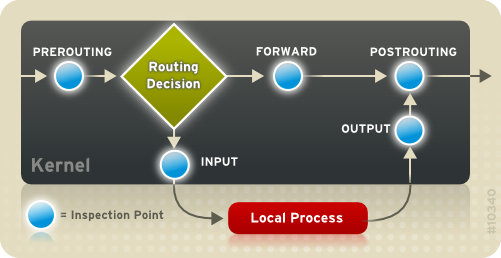
\includegraphics[width=0.8\linewidth]{iptables_small}
  \end{center}
  \vfill
\end{frame}


\begin{frame}
  \frametitle{Tables (iptables)}

  \vfill

  \begin{block}{But}
    \begin{itemize}
    \item organisation du traitement suivant le but recherché
    \item pour la sécurité, on s'intéresse surtout à la table
      \texttt{filter}
    \item c'est la table par défaut
    \end{itemize}
  \end{block}
  \vfill
  \begin{block}{Spécification}
    \begin{itemize}
  \item \texttt{-t nom}
  \item \texttt{mangle}: changement des paquets
  \item \texttt{nat}: Network Address Translation, voir plus loin
  \item \texttt{security}: MAC avec SELinux
  \item Il est possible de créer d'autres tables
    \end{itemize}
  \end{block}
  \vfill
\end{frame}

\begin{frame}
  \frametitle{Chaînes}

  \vfill
  \begin{block}{Chaînes de la table \texttt{filter}}
    \begin{itemize}
    \item INPUT: traitement des paquets destinés à la machine courante
    \item OUTPUT: traitement des paquets issus de la machine courante
    \item FORWARD: traitement des paquets passant seulement à travers
      la machine courante (passerelle)
    \end{itemize}
  \end{block}
  \vfill
  \begin{block}{Fonctionnement des chaînes}
    \begin{itemize}
    \item chaque chaîne est une liste de règles
    \item on peut ajouter une règle au début d'une chaîne avec \texttt{-I chaine}
      ou à la fin avec \texttt{-A chaine}
    \item la première règle applicable est choisie en partant du début
    \end{itemize}
  \end{block}
  \vfill
\end{frame}


\begin{frame}
  \frametitle{Règles}
  \vfill

  \begin{block}{Principe}
    \begin{itemize}
    \item chaque règle est associée à une chaîne dans une table 
    \item elle décrit les caractéristiques des paquets auxquels elle
      va s'appliquer (\textit{cf.} planches précédentes)
    \item elle contient l'action à effectuer lorsque les conditions
      sont remplies par le paquet
    \item spécification d'une action:  \texttt{-j action}
    \end{itemize}
  \end{block}
  \vfill
  \begin{block}{Actions spécifiques pour le filtrage}
    \begin{itemize}
    \item \texttt{accept}: laisse passer le paquet
    \item \texttt{reject}: bloque le paquet et signale le blocage par
      un paquet ICMP \emph{destination unreachable}
    \item \texttt{drop}: bloque silencieusement le paquet
    \end{itemize}
  \end{block}
  \vfill
\end{frame}

\begin{frame}
  \frametitle{Exemple}
  \vfill
  \begin{block}{But}
    interdire l'accès au réseau servi par eth0 à partir de l'extérieur (connecté à eth1)
  \end{block}
  \pause\vfill 
  \begin{block}{Première version}
    \small\tt iptables -I FORWARD -i eth1 -o eth0 -j REJECT
  \end{block}
   \pause\vfill 
 \begin{block}{Seconde version (n'empêche pas les réponses)}
    \small\tt iptables -I FORWARD -m state -\,-state NEW -i eth1 -o eth0 -j REJECT
  \end{block}
   \pause\vfill 
 \begin{block}{Autorise l'accès à une machine (règle à évaluer avant)}
    \small\tt iptables -I FORWARD  -i eth1 -d 10.0.0.2 -j ACCEPT
  \end{block}
  \vfill
\end{frame}


\begin{frame}
  \frametitle{La table NAT}
  \vfill
  \begin{block}{Utilisation}
    \begin{itemize}
    \item Partager une adresse IP entre plusieurs machines d'un réseau interne
    \item Exemple d'utilisation: box internet
    \item Sécurité:
      \begin{itemize}
      \item permettre aux machines du réseau local de se connecter à
        Internet
      \item mais par manque d'adresse publique, il est impossible à
        une machine externe d'initier une connexion vers une machine
        du réseau interne
      \end{itemize}
    \end{itemize}
  \end{block}
  \vfill
  \begin{block}{Commande}
    \small\tt iptables -t nat -A POSTROUTING -o eth1 -j MASQUERADE
  \end{block}
\end{frame}
  
\end{reveals}
\end{document}
 
